\documentclass[conference]{IEEEtran}
\usepackage[T1]{fontenc}
\usepackage{array}
\usepackage{calc}
\usepackage{multirow}
\usepackage{color}
\usepackage{amsthm}
\usepackage{amssymb}
\usepackage[normalem]{ulem}
\usepackage{graphicx}
\usepackage{breakurl}
\usepackage[compact]{titlesec}
\titlespacing{\section}{9pt}{8pt}{4pt}
\titlespacing{\subsection}{7pt}{5pt}{1pt}
\titlespacing{\subsubsection}{1pt}{1pt}{*0}
\setlength{\skip\footins}{0.2cm}
\makeatletter

\usepackage[font=small]{caption} 

\providecommand{\tabularnewline}{\\}

 \let\oldforeign@language\foreign@language
 \DeclareRobustCommand{\foreign@language}[1]{%
   \lowercase{\oldforeign@language{#1}}}
\theoremstyle{plain}
\newtheorem{thm}{\protect\theoremname}
\theoremstyle{plain}
\newtheorem{conjecture}[thm]{\protect\conjecturename}


\ifCLASSOPTIONcompsoc

\usepackage[caption=false,font=normalsize,labelfont=sf,textfont=sf]{subfig}
\else
\usepackage[caption=false,font=footnotesize]{subfig}
\usepackage{multicol}


\fi

\providecommand{\conjecturename}{Hypothesis}
\providecommand{\theoremname}{Theorem}


\newcommand\petko[1]{#1}  

\newcommand{\red}[1]{{#1}}
\newcommand{\rv}[1]{}

\makeatother

\clubpenalty = 10000
\widowpenalty = 10000
\displaywidowpenalty = 10000

\begin{document}

\title{Improving SOA Antipatterns Detection in Service Based Systems by Mining Execution Traces}

\author{Mathieu Nayrolles, Naouel Moha, and Petko Valtchev\\
LATECE Team, D\'epartement d'informatique, Universit\'e du Qu\'ebec \`a Montr\'eal, Canada\\
mathieu.nayrolles@gmail.com, \{moha.naouel,valtchev.petko\}@uqam.ca}

\maketitle
\thispagestyle{empty}

\begin{abstract}

Service Based Systems (SBSs), like other software
systems, evolve due to changes in both user requirements and
execution contexts. Continuous evolution could easily deteriorate
the design and reduce the Quality of Service (QoS) of SBSs and
may result in poor design solutions, commonly known as SOA
antipatterns. SOA antipatterns lead to a reduced maintainability and
reusability of SBSs. It is therefore important to first detect and
then remove them. However, techniques for SOA antipattern
detection are still in their infancy, and there are hardly any tools
for their automatic detection. In this paper, we propose a new
and innovative approach for SOA antipattern detection called SOMAD
(Service Oriented Mining for Antipattern Detection) which is an evolution of the previously published SODA \red{(Service Oriented Detection For Antpatterns)} tool. 
SOMAD improves SOA antipattern detection by mining execution traces:
It detects strong associations between sequences of service/method calls and further filters them using a suite of dedicated metrics. We first present the underlying association mining model and introduce
the SBS-oriented rule metrics. We then describe a validating
application of SOMAD to two independently developed SBSs. A comparison of our new tool with SODA reveals superiority of the former: Its precision is better by a margin ranging from 2.6\% to 16.67\% while the recall remains optimal at 100\% and the speed is significantly reduces (2.5+ times on the same test subjects).

\end{abstract}
\begin{IEEEkeywords}
SOA Antipatterns, Mining Execution Traces, Sequential Association Rules, Service Oriented Architecture.
\end{IEEEkeywords}



\section{Introduction}

Service Based Systems (SBSs) are composed of ready-made services that are accessed through the Internet~\cite{erl2006service}. Services
are autonomous, interoperable, and reusable software units that can be implemented
using a wide range of technologies like Web Services, REST (REpresentational
State Transfer), or SCA (Service Component Architecture, on the top of SOA.). Most of
the world's biggest computational platforms: Amazon, Paypal, and eBay, for example, represent large-scale SBSs. Such systems are complex--they may generate massive flows of
communication between services--and highly dynamic: services appear, disappear or get modified.
The constant evolution in an SBS can easily deteriorate the
overall architecture of the system and thus bad design choices, known as SOA \textit{antipatterns}~\cite{Moha12-ICSOC-SOASpecificationDetection}, may appear.
An antipattern is the opposite of a design pattern: while
patterns should be followed to create more maintainable and reusable
systems~\cite{wolfgang1994design}, antipatterns must be avoided
since they have a negative impact, e.g., hinder the maintenance and reusability of SBSs.

Given their negative impact, there is a clear and urgent need for techniques and tools to detect SOA antipatterns. Recently, a tool was developed by our team, called SODA (Service Oriented Detection for Antipatterns)~\cite{Moha12-ICSOC-SOASpecificationDetection,Nayrolles12-ICSOC-SODA}, which targets SOA antipatterns. The tool employs a Domain Specific Language (DSL) to specify SOA antipatterns, which is based on metrics and generates detection algorithms from antipattern specifications in an automated way.

Albeit efficient and precise, SODA suffers from serious limitations. Indeed, the tool performs two phases of analysis, first, a static one and then a dynamic one. The static analysis requires access to service interfaces. Consequently, SODA cannot analyze systems that are proprietary or not open-source. The dynamic analysis requires the execution of the system and therefore, the creation of runnable scenarios. Moreover, since SODA 
specifically targets systems implementing the SCA standard, its precision drops as the target system gets bigger. 
%
Given these limitations, there is a space for improvement, both in precision and in coverage, i.e., detection of antipatterns in SBSs implementing a wider range of SOA technologies.
%
In this article, we propose a new and innovative approach for the detection of SOA antipatterns named SOMAD (Service Oriented Mining for Antipattern Detection). SOMAD does not require scenarios to concretely invoke service interfaces as it only relies on execution traces (provided by any SOA technology). It discards irrelevant data by using data mining techniques--sequential association rules mining--. The tool discovers SOA antipatterns by first extracting associations between services as expressed in the execution traces of an SBS. To that end, it applies a specific variant of the association rule mining task based on sequences or episodes: In our case the sequences represent service or, alternatively, method calls. Further on, generated association rules are filtered using a suite of dedicated metrics.

We applied SOMAD on two different SBS called \emph{Home Automation} and \emph{FraSCAti}~\cite{SPE:SPE1077}. \emph{Home Automation} is made of 13 services and \emph{FraSCAti} is almost ten times larger. We compared the outcome of SOMAD to the one produced by SODA, the so far unique tool for SOA antipatterns detection from the literature. Both tools were evaluated in terms of precision and recall, on one hand, and efficiency, on the other hand.  The study results indicate that SOMAD significantly outperforms SODA in term of precision (2.6\% to 16.67\%) and efficiency (2.5+ times faster).

The main contribution of this paper is thus twofold: (i) a new approach for the detection of SOA antipatterns based on association rules mining from the execution traces of an SBS (from a variety of SOA technologies); (ii) an empirical validation of this approach, which shows the tool outperforms its direct competitor in terms of precision and efficiency. 

The remainder of the article is organized as follows. Section~\ref{sec:related-work} presents related works on pattern and antipattern detection both in SOA and OO paradigms and related works on knowledge extraction. Section~\ref{sec:Methodology}
presents the SOMAD approach, and in particular the mining of association rules from execution traces while, Section~\ref{sec:Experimentation} presents our experimental study with a comparison of our SOMAD approach to SODA. Finally, we provide some concluding remarks in Section~\ref{sec:Conclusions}.


\section{Related Work} \label{sec:related-work}

As our approach combines antipattern detection and knowledge extraction from execution traces we provide short serveys of related work on both: Section~\ref{sec:motifs} deals with detection of patterns and antipatterns  both in OO and SOA paradigms while Section~\ref{arm} addresses knowledge extraction. Finally, Section~\ref{SODA} presents the SODA approach~\cite{Moha12-ICSOC-SOASpecificationDetection,Nayrolles12-ICSOC-SODA}.

%Our approach relates to two different fields: antipattern detection and execution log mining.
\subsection{Pattern and Antipattern Detection \label{sec:motifs}}


Architectural (or design) quality is essential for building well-designed,
maintainable, and evolvable SBSs. Patterns --and antipatterns-- have been
recognized as one of the best ways to express architectural concerns
and solutions, and thus target high quality in systems. 
A number of methods and tools exist for the detection of antipatterns in OO systems~\cite{Kessentini10-ASE-Deviance,Lanza06-OOMetricsPractice,Moha:2010:DMS:1729475.1729592}
%and correction \cite{DuBois04-WCRE-RefactoringCouplingCohesion},\cite{Simon01-CSMR-MetricsBasedRefactoring},\cite{Trifu03-StrategyBasedDesignFlaws}
whereas the relevant theory and practices have been summarized in best-sellers books~\cite{Brown98-AntiPatterns,kentbeck}. However, the detection of SOA antipatterns, unlike their OO counterparts, is still in its infancy. 
%

An approach to the declarative specification of antipatterns, called SPARSE, is presented in~\cite{Settas:2011:SSA:1943774.1943847}. In SPARSE, antipatterns are described as an OWL ontology augmented with
a SWRL (Semantic Web Rule Language) rule basis whereas their occurrences are tested through automated reasoning.  

%For example, Brown \emph{et al.}~\cite{Brown98-AntiPatterns}
%introduced a collection of 40 antipatterns, Beck, in Fowler's highly-acclaimed
%book on refactoring~\cite{kentbeck}, compiled 22 code smells that
%are low-level antipatterns in source code, suggesting where engineers
%should apply refactorings. One of the root causes of OO antipatterns
%is believed to be the adoption of a procedural design style in OO systems.
%For SOA antipatterns, in turn, it is rather the adoption of an OO design style
%in SOA systems~\cite{Kral07-SOAAntipatterns}.

%Despite a number of commonalities, OO antipattern detection methods and tools cannot be directly applied to SOA.
%Indeed, SOA focuses on services as first-class entities whereas OO focuses on classes,
%which are at a lower level of granularity. Moreover, the highly
%dynamic nature of an SOA environment raises several challenges that
%are not faced in OO development. In particular, it requires dynamic analysis.

Other relevant work has focused on the detection of specific antipatterns
related to the system's performance and resource usage and/or given technologies.
For example, Wong \emph{et al.}~\cite{Wong:2010:REU:1919284.1919587}
use a genetic algorithm for detecting software faults and anomalous
behavior in the resource usage of a system (e.g. memory usage,
processor usage, thread count). The approach is driven by \emph{utility
functions} that correspond to predicates identifying suspicious
behavior by means of resource usage metrics.
%For example, a utility function
%may report an anomalous behavior corresponding to spam sending if
%it detects a large number of threads.
In another related work, Parsons \emph{et al.}~\cite{Parsons_detectingperformance}
tackled the detection of performance antipatterns.
They use a rule-based approach made of both static and dynamic analyzes
that are tailored to component-based enterprise systems (in particular, JEE applications).

\subsection{Knowledge Extraction\label{arm}}
A large number of studies focused on knowledge extraction from execution traces.
They were motivated by the identification of:
crosscutting concerns (aspects)~\cite{Tonella04-WCRE-AspectMining}, %by means of formal concept analysis
business processes~\cite{Khan:2009:APM:1926618.1926651}, 
patterns of interests among service users%usage patterns and behaviors among web services usage and interactions
~\cite{Asbagh:2007:WSU:1348171.1348217,Dustdar:27February2007:1741-8763:256},
%i.e. find sequences of web service operations which are called by web service users
%This yields in hand knowledge about the patterns of interests
%among service users and indicates that which services
%have high correlation with each other.
and features either in OO systems~\cite{10.1109/ICPC.2006.19} or SBSs~\cite{conf/icsm/YousefiS11}.
% study the mining of dynamic call trees for the identification of distributed features in an SOA environment.
Further related work focused on the identification of service composition patterns \cite{Upadhyaya12-JSEP-MiningServiceComposition}, i.e. sets of services that are repetitively used together in different systems and that are structurally and functionally similar.
Composition patterns embody good practices in designing and developing SBSs.


Few projects have explored pattern detection through execution trace mining. Ka-Yee Ng \emph{et al.} \cite{ng2010identification} proposed MoDeC, an approach for identifying behavioral and creational design patterns using dynamic analysis and constraint programming. They reverse-engineer scenario diagrams from an OO system by bytecode instrumentation and apply constraint programming to detect these patterns as runtime collaborations.
%MoDeC consisted in reverse-engineering an OO system in the form of scenario diagrams by means of dynamic analysis through bytecode instrumentation. Then, the patterns were identified in scenario diagrams as runtime collaborations among objects by means of constraint programming. 
Hu and Sartipi~\cite{Hu08-SEKE-DynamicAnalysis} tackle the detection of design patterns in traces using scenario execution, pattern mining, and concept analysis. The approach is guided by a set of feature-specific scenarios to identify patterns, as opposed to a general pattern detection.
%These works targeted OO systems and patterns as good practices.


Although different in goals and scope, the above studies on OO antipatterns form a sound basis of expertise and technical knowledge for building methods for the detection of SOA antipatterns. However, despite a large number of commonalities, OO (anti)pattern detection methods cannot directly apply to SOA. Indeed, SOA focuses on services as first-class entities and thus remains at a higher granularity level than OO classes. Moreover, the highly dynamic nature of a SBS raises challenges that are not preponderant in OO systems.  

%.------

%\naouel{� ajouter : \cite{Settas:2011:SSA:1943774.1943847} ?}
%\naouel{� revoir, pas acc�s � l'article: Also Liang \emph{et al.}~\cite{LIANG:2006:SPD:1190612.1190926} look after
%service patterns in web services at different level and in particular at user level.}
%\petko{Article sur le site (r�p. Rel. Work)}

%\cite{Upadhyaya12-JSEP-MiningServiceComposition}
%Abstract: We locate a set of associated services using Apriori algorithm and recover the control flows among the services by analyzing the order of service invocation events in the execution logs. We also identify structurally and functionally similar patterns to represent such patterns in a higher level of abstraction regardless of the actual services
%
%Bipin et al, for their parts use mining techniques to detect patterns
%in service composition and deal with the identification of
%different types of structural similarity. Structural similarity
%is also the cornerstone of our work.

%Upadhyaya \emph{et al.}~\cite{upadhyaya2012approach} use mining techniques
%to detect patterns in service composition and identify different types of structural
%similarity. Structural similarity is also the cornerstone of our work.
%
%----------------------------
%Anis Yousefi and Kamran Sartipi [25] have mine dynamic call tree for identifying distributed
%features in an SOA environment and Figure out how to deal
%with the distributed locations of execution logs.

%Abstract : In this paper, we propose a new approach for identifying the implementation
%of web service features in a service oriented architecture (SOA)
%by mining dynamic call trees that are collected from distributed
%execution traces.
%

\subsection{SODA : The State-of-the-Art Tool\label{SODA}}

%As mentioned earlier, the only approach currently available is SODA~\cite{Moha12-ICSOC-SOASpecificationDetection, Nayrolles12-ICSOC-SODA}. 
SODA relies on a rule-based language that enables antipatterns specification using a set of metrics. A generic process then turns the specification into detection algorithms. The three main steps of the processing are as follows (see Figure~\ref{fig:The-SODA-approach}):

\begin{figure*}
\framebox{\begin{minipage}[t]{1pt + 2\columnwidth}%
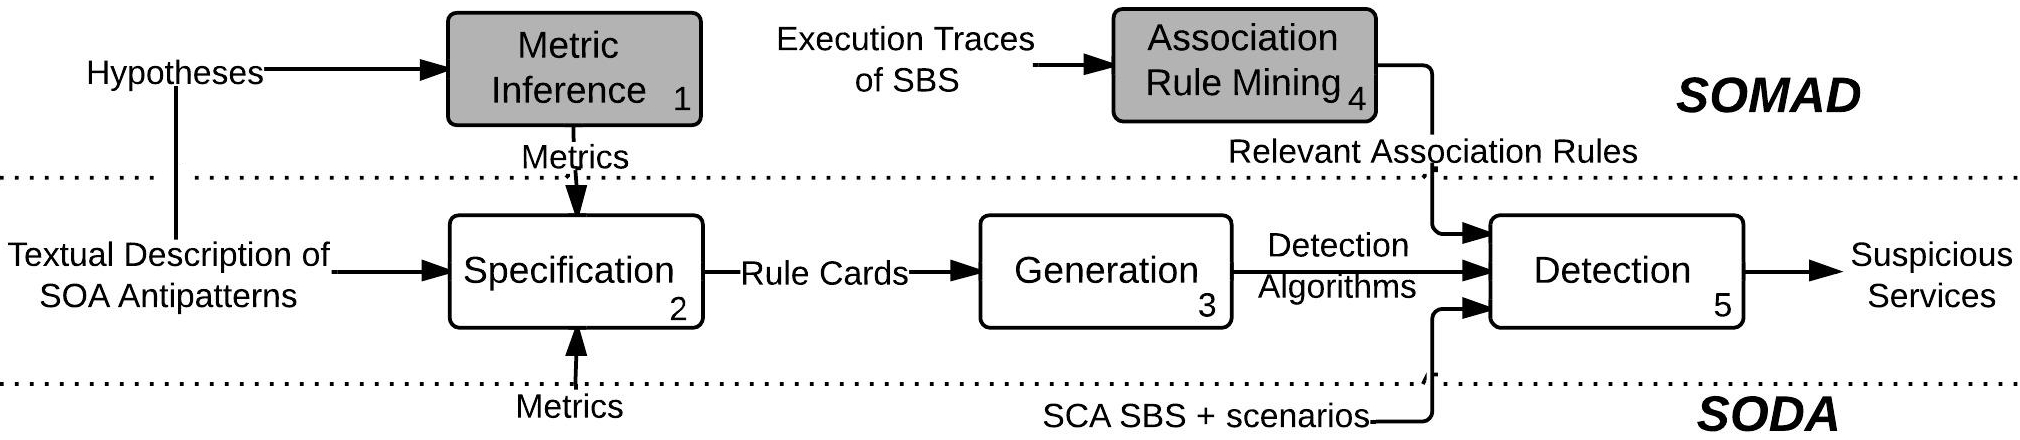
\includegraphics[scale=0.25]{media/SODA.png}%
\end{minipage}}
\caption{\label{fig:The-SODA-approach}SODA and SOMAD approaches: Grey boxes depict new steps in SOMAD w.r.t. to SODA (white boxes).}
\end{figure*}

\emph{Specification of SOA Antipatterns}: Relevant properties of SOA antipatterns are identified, which essentially correspond to metrics such as cohesion, coupling, number of methods, response time and availability. These properties compose to a base vocabulary of a DSL: a rule-based language is used whereby each rule expresses tendencies in metric values. An antipattern is described by a set of rules combined into a \textit{rule card}.

\vspace{0.12cm}

\emph{Generation of Detection Algorithms}: Automatic generation of detection algorithms is performed by visiting models of rule cards specified during the previous step. The process is straightforward and ends up with a set of directly executable algorithms.
%The generation process relies on Java code templates that correspond to the detection algorithms. .

\vspace{0.12cm}

\emph{Detection of SOA Antipatterns}: The detection algorithms generated in the previous step are applied on the SBS of interest. This step allows the automatic detection of SOA antipatterns using a set of predefined scenarios to invoke service interfaces. At the end, services from the SBS suspected of being involved in an antipattern are identified.

\vspace{0.15cm}

Although efficient and precise, SODA is an intrusive approach because it requires a set of valid scenarios concretely invoking the interface methods of SBSs and its dynamic analysis involves SCA properties. 

%
%\textcolor{blue}{\emph{Step 1. Specify SOA antipatterns:} This step lies in identifying properties in SBSs relevant to SOA antipatterns. 
%To achieve the specification we perform a thorough domain analysis of SOA antipatterns by analyzing their definitions and specification in the literature to identify relevant properties. These properties are used as a base vocabulary (Cohesion, Coupling, ...) to a DSL, in the form of a rule-based language for specifying antipatterns.}
%
%\textcolor{blue}{\emph{Step 2. Generate detection algorithms: }In this step, detection algorithms are generated automatically from the specifications defined in the previous step. Using the previous specification and our DSL; we implemented the generations as a set of visitors on models of the antipatterns rule card (rule cards are combination of rules). These algorithms are directly executable.} 
%
%\textcolor{blue}{\emph{Step 3. Detection: }Detect automatically SOA antipatterns: The third step consists of applying, on the SBSs of interest, the detection algorithms generated in \emph{Step 2} to detect SOA antipatterns.}


\section{The SOMAD Approach \label{sec:Methodology}}



We propose a five step approach, named SOMAD (Service Oriented Mining for Antipatterns Detection), for the detection of SOA antipatterns within execution traces of SBSs. This new approach is a variant of SODA based on execution traces, which may come from any kind of SBSs. 
In contrast, SODA applies specifically on SCA SBSs using a set of scenarios and SCA-based techniques. In particular, in SOMAD, we specify a new set of metrics that apply to sequential association rules mined on execution traces whereas, in SODA, metrics apply to the concrete invocation of SBSs' interfaces using a set of scenarios. 
%As a result, the detection of SOA antipatterns with SOMAD is non-intrusive and technology agnostic because it only requires execution traces.
Figure \ref{fig:The-SODA-approach} shows an overview of SOMAD. We emphasized in grey the two new steps specific to SOMAD and added to the SODA approach. \textit{Step~1. Metric Inference} is supported by the creation of a set of hypotheses made from the textual description of SOA antipatterns. The hypotheses underlie the definition of new  metrics to support the interpretation of association rules. \textit{Step~4. Association Rule Mining} (ARM) discovers interesting sequential associations in execution traces of the targeted SBS. \rv{2-2} Output sequential association rules represent \red{statistically} interesting relations between services inside traces. In what follows, we first introduce key concepts of sequential ARM and then, present the overall process of SOMAD. Finally, we provide some implementation details.

\subsection{Introduction to Sequential Association Rule Mining}

\noindent In the data mining field, ARM is a
well-established method for discovering co-occurrences between attributes
in the objects of a large data set~\cite{piatetsky1991discovery}. Plain
associations have the form $X \rightarrow Y$, where $X$ and $Y$,
called the \textit{antecedent} and the \textit{consequent}, respectively, are sets of descriptors
(purchases by a customer, network alarms, or any other general kind of events).
Even though plain association rules could serve some relevant information, we are interested here in
the sequences of service invocations.
We therefore adopt a variant called sequential association rules in which
both $X$ and $Y$ become sequences of descriptors.
Moreover, our sequences follow a temporal order with the antecedent preceding the consequent. 
Rules of this type mined from traces reveal crucial
information about the likelihood that services appear together in an execution
trace and, more importantly, in a specific order. 
For instance, a strong rule \emph{ServiceA $,$ ServiceB } implies \emph{ServiceC} would mean that after executing A and then B, there are good chances to see C in the trace.
The conciseness of this example should not confuse the reader as in practical cases
the sequences appearing in a rule can be of an arbitrary length.
Furthermore, the strength of the rule is measured by the \textit{confidence} metric: In probabilistic terms,
it measures the conditional probability of C appearing down the line.
Beside that, the significance of a rule, i.e. how many times it appears in the data,
is provided by its \textit{support} measure.
To ensure only rules of potentially high interestingness are mined,
the mining task is tuned by minimal thresholds to
output only the sufficiently high scores for both metrics.



\subsection{SOMAD Process}


\noindent \emph{Step 1. Metrics Inference:} Metrics to support the interpretation of sequential association rules are inferred from a set of three hypotheses synthesized from the textual description of SOA antipatterns (Table~\ref{tab:List-of-SOA}).
\vspace{0.15cm}
\\
\noindent These hypotheses represent heuristics that enable the identification of \red{architectural} properties relevant to SOA antipatterns. Indeed, after a careful examination of the textual descriptions, we observed that SOA antipatterns can be specified in terms of coupling and cohesion\footnote{Recall coupling basically refers to the degree a services relies on others while cohesion measures the relatedness between its own responsibilities~\cite{stevens1974structured}.}.

%\noindent \textcolor{blue}{In order to infer new metrics able to identify SOA antipatterns properties highlighted from their textual description in ; we need hypotheses helping us to match these properties against the encoded sequential association rules information. These hypothesis work as a kind of heuristic to interpret sequential association rules in order to identify properties relevant to SOA antipatterns. After a careful examination of antipattern textual description, we observe that many of them reflect a high degree of coupling to other services\footnote{The
%coupling basically refers to the degree a services relies on others~\cite{stevens1974structured}.}.
%We therefore conclude that such antipatterns can be defined, at least partially,
%in terms of incoming and outgoing coupling.}



%\noindent To accomplish the detection of antipatterns given in Table~\ref{tab:List-of-SOA} ) we have to decode the sequential association rules information. As described before, a sequential association rule indicates how likely
%is a set of services to be called together in the specific order defined by the rule\footnote{In fact,
%how likely a sequence of services/methods (the rule consequent) is to occur after observing another sequence (the antecedent).}.
%To detect SOA antipatterns within sequential association rules we need to make hypotheses; the key idea behind them is to identify SOA antipatterns properties, such as cohesion or coupling, while analysing sequential association rules rather than service interfaces. 



% in this non-common allegory. Newly created hypothesis are then used to infer metrics able to measure SOA antipatterns properties, for example the cohesion, coupling and number of methods inside the sequential association rules.

\begin{table}
\caption{List of SOA Antipatterns \cite{Moha12-ICSOC-SOASpecificationDetection} \label{tab:List-of-SOA}}
\begin{tabular*}{8.7cm}{@{\extracolsep{\fill}}p{8.7cm}}
\tabularnewline
\textbf{Multi-Service}, \textit{a.k.a} God Object corresponds to a service
that implements a \textbf{multitude of methods} related to different
business and technical abstractions. This aggregate too much into
a single service, such a service is not easily reusable because of
the \textbf{low cohesion} of its methods and is often unavailable
to end-users because of its overload, which may induce a high response
time \cite{Dudney03-J2EEAntipatterns}.\tabularnewline
\noalign{\vskip0.15cm}
\textbf{Tiny Service} is a small service with\textbf{ few methods}, which only
implements part of an abstraction. Such service often requires \textbf{several
coupled services} to be used together, resulting in higher development
complexity and reduced usability. In the extreme case, a Tiny Service
will be limited to \textbf{one method}, resulting in many services
that implement an overall set of requirements \cite{Dudney03-J2EEAntipatterns}.\tabularnewline
\noalign{\vskip0.15cm}
\textbf{Chatty Service} corresponds to a set of services that exchange a \textbf{lot
of small data} of primitive types. The Chatty Service is also characterized
by a\textbf{ high number of method invocations}. Chatty Service chats
a lot with each other \cite{Dudney03-J2EEAntipatterns}.\tabularnewline
\noalign{\vskip0.15cm}
\textbf{The Knot} is a \textbf{set of very} \textbf{low cohesive} services,
which are tightly coupled. These services are thus less reusable.
Due to this complex architecture, the availability of these services
can be low, and their response time high \cite{ArnonSOARotem11-SOAPatterns}.\tabularnewline
\noalign{\vskip0.15cm}
\textbf{Bottleneck Service} is a service that is \textbf{highly used} by other
services or clients. It has a \textbf{high incoming and outgoing coupling}.
Its response time can be higher because it may be used by too many external
clients, for which clients may need to wait to get access to the service.
Moreover, its availability may also be low due to the traffic.\tabularnewline
\noalign{\vskip0.15cm}
\textbf{Service Chain}, a.k.a. Message Chain in OO systems, corresponds
to a \textbf{chain of services}. The Service Chain appears when clients
request \textbf{consecutive service invocations} to fulfill their
goals. This kind of \textbf{dependency chain} reflects the action
of invocation in a transitive manner.
\tabularnewline
\end{tabular*}\end{table}

\begin{conjecture}
If a service A \emph{implies} a service B with a high support and a high confidence, then
A and B are tightly coupled.
\end{conjecture}

\begin{conjecture}
If a service appears in the consequent (antecedent) parts for a high number of associations,
then it has high incoming (outgoing) coupling.
\end{conjecture}

\noindent The above hypotheses qualify the coupling between two specific
services and overall incoming/outgoing coupling. The cohesion is also widely used in
SOA antipattern descriptions. 
%\begin{conjecture}
%\sout{If the number
%of different methods of a given service is
%similar to the number of different partners (Hypothesis 2) it has
%in the service rules,
%then the service is not cohesive.}
%\end{conjecture}
\begin{conjecture}
\rv{1-1} \rv{2-3} \rv{3-1} \red{If the number
of different methods of a service A is
equal or superior to the number of different services invoking A (Hypothesis 2) 
then, the service is not externally cohesive.}
\end{conjecture}

\noindent \red{This definition of cohesion has been introduced by Perepletchikov \textit{et al.}: "\textit{A service is deemed to be Externally cohesive when all of its service operations are invoked by all the clients of this service}" \cite{Perepletchikov2010}}. Based on the above three hypotheses, we have created domain specific metrics
to help us explore the antipattern manifestations that are hidden in the sequential association rules. We use the DSL we defined in~\cite{Moha12-ICSOC-SOASpecificationDetection} to combine them. Metrics are presented in Table~\ref{tab:metrics}. In the
figure, standard mathematical notations are used whenever possible
and extended if necessary. Thus, association rules are visualized
by (X $\rightarrow$ Y) with X and Y represent the antecedent and
the consequent parts, respectively. \emph{K, L} are partner services.
$AR$ stands for the overall set of association rules while $AR_{s}$
and $AR_{m}$ being subsets targeting association rules at service / method level, respectively. \emph{$M_{S}$}
denotes the methods of a given service $S$. Finally, we use non-standard
symbols for sequence operations: $[ ]$ is the sequence constructor,
$\Cup$ stand for append on sequences; $\Subset$ denotes the sub-sequence-of
relationship; and A $\lessdot$ B means the service/method A appears
inside \red{the association rule B}. Metrics can be combined to define other metrics.

\begin{table*}
\caption{Metrics $\Cup$ : append on sequences; $\Subset$ : sub-sequence-of relationship; and A $\lessdot$ B : A appears inside B.\label{tab:metrics}}
{\renewcommand{\arraystretch}{1.5}}
\begin{tabular}{|>{\normalsize}p{2\columnwidth}|}
\hline
\textbf{\textit{Number of Matches (NMA(S))}} : $\#\{X\rightarrow Y\in AR_{s}\mid S\lessdot(X\Cup Y)\}$ \\ 
Follows the number of rules where a service appears, either on the left- or on the right-hand side. \\ \hline \hline
\textbf{\textit{Number of Diff. Partners (NDP(S))}} : $\#\{K\mid X\rightarrow Y\in AR_{s},S\lessdot X,K\lessdot Y\}$
  $+~\#\{K\mid X\rightarrow Y\in AR_{s},S\lessdot Y,K\lessdot X\}$ \\ 
Indicates how many different partners a service
has. Spelled differently, the metric determines whether the
service communicates intensively with surrounding services
or not. \\ \hline \hline
\textbf{\textit{Number of Methods (NM(S))}} : $\#\{K\mid X\rightarrow Y\in AR_{m},K\in M_{s},K\lessdot(X\Cup Y)\}$ \\ 
Counts
the number of occurrences of the methods from a service.
The counting for this metric focuses on method rules.
 \\ \hline \hline 
\textbf{\textit{Cohesion (COH(S))}} : $\frac{NDP(S)}{NM(S)}$ \\ 
Assesses the ratio
between the numbers of partner services and of the available
methods, respectively. \\ \hline \hline
\textbf{\textit{Cross Invocation Dependencies (CID($S_{a},S_{b}$))}} : $\#\{X\rightarrow Y\in AR_{s}\mid S_{a}\lessdot X,S_{b}\lessdot Y\}$ $+~ \#\{X\rightarrow Y\in AR_{s}\mid S_{a}\lessdot Y,S_{b}\lessdot X\}$  \\ 
\red{CID is a keystone of the SOMAD approach}. Indeed, the metric would explore the typical
interactions between services while ignoring less frequent
ones (absent from the mining method output due to the
support threshold). To retrieve this information CID counts
all association rules where a service A (Sa) is present in
the antecedent and a service B (Sb) in the consequent or
\textit{vice versa}. \\ \hline \hline
\textbf{\textit{Incoming Coupling (IC(S))}} : $\sum_{L\in\{K\mid X\rightarrow Y\in AR_{s},K\lessdot X,S\lessdot Y\}}\frac{CID(S,L)}{NDP(S)}$ \\ 
Counts how many times a service is used.
Yet instead of merely counting a unit for each partner service, we
use a contextual value: $\frac{CID(S,X)}{NDP(S)}$ where $X$ is the
partner service. Thus, the larger the portion of the partner service
in the overall number of partners of $S$, the higher the coupling. \\ \hline \hline
\textbf{\textit{Outgoing Coupling (OC(S))}} : $\sum_{L\in\{K\mid X\rightarrow Y\in AR_{s},S\lessdot X,K\lessdot Y\}}\frac{CID(L,S)}{NDP(S)}$ \\ 
The same principle as for \textbf{IC}, yet applied in
a dual manner: counts how many times the argument service
uses other ones. \\ \hline \hline
\textbf{\textit{Transitive Coupling (TC$(S_{a},S_{b})$)}} : $\#\{K\mid X\rightarrow Y\in AR_{s},S_{a}\lessdot X,S_{b}\lessdot Y,({[S_{a},K]\Subset X}\vee[K,S_{b}]\Subset Y)\}$ \\ 
Metric targets the \textit{Service Chain} SOA antipattern 
(see above). First, observe that the founding idea of \textit{Service Chain}
is that absence of direct communication between a pair of services
does not mean zero coupling.
To identify transitive coupling manifestations 
we need to capture the notion of a chain: e.g. a service $S_{a}$ is
in the antecedent of a rule, another one $S_{b}$ is in the consequent of another
rule and both rules are connected by means of a third service $K$
that appears in the consequent of the first rule and in the antecedent
of the second one. Longer chains are possible as well. Thus, in the
basic case, one could have {[}A{]}$\rightarrow${[}B{]} and {[}B{]}$\rightarrow${[}C{]}.
In this configuration, although A and C are not directly coupled, if C
fails, there are good chances that A (and B) would fail too.
\\ \hline 

\end{tabular}
\end{table*}


\vspace{0.10cm}

\noindent \emph{Step 2. Specification of SOA Antipatterns:} The combination of metrics defined in the previous step allows the specification of SOA antipatterns in the form of sets of rules, called \textit{rule cards}.
\vspace{0.15cm}
\\
\noindent For the individual
metrics and combinations thereof, the values that trigger the detailed
examination of a case are not fixed beforehand. Instead, we use a
boxplot-based statistical technique that exploits the distribution
of all values across the sets of services, methods, and rules. Moreover,
the computed values are further weighted using the quality metrics
for associations, i.e. support and confidence, so that the strongest
rules could be favored. The \textit{rule cards} used to specify SOA  antipatterns are presented in Figure~\ref{fig:rules}. As an example, the rule card corresponding to the Tiny Service specification (Figure 3(b)) is composed of three rules. The first one (line 2) is the intersection of two rules (lines 3, 4), which define two metrics: a high Outgoing Coupling (OC) and a low Number of Method (NM).
%We determine if a value it's high or not with the boxplot statistical
%method. A boxplot distinguish differences between population of values
%using their statistical distribution. Thus, using this technique,
%we don't have to set subjective thresholds to detect antipatterns.
%Moreover, the values are weighted by $\frac{support}{confidence}$
%for highlighting most confident and supported association rules.
%The rule cards used to detect the individual antipatterns are as
%follows. %We now present how these metrics based on our conjectures can match
%%the textual description of SOA antipatterns.
%\textit{Multi-service} is signaled whenever high values of \textbf{NMA} and
%\textbf{NM} co-occur with low values of \textbf{COH}. For \textit{Tiny service}, high
%values of \textbf{OC} with low values of \textbf{NM} are indicative. Very high values
%of \textbf{NMA} and \textbf{NPD} (i.e. outliers in the boxplot), correspond to the \textit{Chatty service} while \textit{Bottleneck} is characterized
%by high values of both \textbf{IC} and \textbf{OC}.  In addition of antipatterns detection describe earlier, we can use our two most complex metrics--\textbf{CID} and \textbf{TC}--to detect other SOA antipatterns. The \textit{Knot} typically involves low values of \textbf{COH}
%combined with high values of \textbf{CID}. Finally,  \textit{Service chain} corresponds
%to the maximal distance between services. Here the distance reflects the (maximal) number of calls necessary to reach one of the services from the other one and it is measured by \textbf{TC}.

\begin{figure}
\begin{small}
\scriptsize
1~RULE\_CARD:~\emph{\textbf{MultiService}}~\{\\
2~~RULE:~\emph{\textbf{MultiService}}\{INTER~\emph{\textbf{LowCohesion}}~\emph{\textbf{ManyMethods}}~\emph{\textbf{ManyMatches}}\};\\
3~~RULE:~\emph{\textbf{LowCohesion}}\{COH~LOW\};\\
4~~RULE:~\emph{\textbf{ManyMethods}}\{NM~HIGH\};\\
5~~RULE:~\emph{\textbf{ManyMatches}}\{NMA~HIGH\};\\
6~\};
\vspace{-0.2cm}
\begin{center}
(a) Multi Service
\end{center}
\vspace{-0.2cm}
1~RULE\_CARD:~\emph{\textbf{TinyService}}~\{\\
2~~RULE:~\emph{\textbf{TinyService}}\{INTER~\emph{\textbf{HighOutgoingCoupling}}~\emph{\textbf{FewMethods}}\};\\
3~~RULE:~\emph{\textbf{HighOutgoingCoupling}}\{OC~HIGH\};\\
4~~RULE:~\emph{\textbf{FewMethods}}\{NM~LOW\};\\
5~\};
\vspace{-0.2cm}
\begin{center}
(b) Tiny Service
\end{center}
\vspace{-0.2cm}
1~RULE\_CARD:~\emph{\textbf{ChattyService}}~\{\\
2~~RULE:~\emph{\textbf{ChattyService}}\{INTER~\emph{\textbf{ManyPartners}}~\emph{\textbf{ManyMatches}}\};\\
3~~RULE:~\emph{\textbf{ManyPartners}}\{NDP~VERY HIGH\};\\
4~~RULE:~\emph{\textbf{ManyMatches}}\{NMA~VERY HIGH\};\\
5~\};
\vspace{-0.2cm}
\begin{center}
(c) Chatty Service
\end{center}
\vspace{-0.2cm}
1~RULE\_CARD:~\emph{\textbf{BottleNeck}}~\{\\
2~~RULE:~\emph{\textbf{BottleNeck}}\{INTER~\emph{\textbf{HighOutgoingCoupling}}~\emph{\textbf{HighIncomingCoupling}}\};\\
3~~RULE:~\emph{\textbf{HighOutgoingCoupling}}\{OC~HIGH\};\\
4~~RULE:~\emph{\textbf{HighIncomingCoupling}}\{IC~HIGH\};\\
5~\};
\vspace{-0.2cm}
\begin{center}
(d) BottleNeck Service
\end{center}
\vspace{-0.2cm}
1~RULE\_CARD:~\emph{\textbf{KnotService}}~\{\\
2~~RULE:~\emph{\textbf{KnotService}}\{INTER~\emph{\textbf{LowCohesion}}~\emph{\textbf{HighCrossInvocation}}\};\\
3~~RULE:~\emph{\textbf{LowCohesion}}\{COH~LOW\};\\
4~~RULE:~\emph{\textbf{HighCrossInvocation}}\{CID~HIGH\};\\
5~\};
\vspace{-0.2cm}
\begin{center}
(e) Knot Service
\end{center}
\vspace{-0.2cm}
1~RULE\_CARD:~\emph{\textbf{ServiceChain}}~\{\\
2~~RULE:~\emph{\textbf{ServiceChain}}\{\emph{\textbf{HighTransitiveCoupling}}\};\\
3~~RULE:~\emph{\textbf{HighTransitiveCoupling}}\{TC~HIGH\};\\
4~\};
\vspace{-0.2cm}
\begin{center}
(f) Service Chain
\end{center}
\end{small}
\vspace{-0.2cm}
\caption{Rule Cards\label{fig:rules}}
\end{figure}

%The first metric, named \textbf{\textit{NMA}}
%(Number of MAtch), follows the number of rules where a service appears,
%either on the left- or on the right-hand side. \textbf{\textit{NDP}}
%(Number of different Partners) indicates how many different partners
%a service has. Spelled differently, the metric determines whether
%the service communicates intensively with surrounding services or
%not. The next pair of metrics is in charge of assessing the coupling,
%or, more precisely, what we call the \textit{incoming coupling} and
%the \textit{outgoing one}. The basic intuition behind \textbf{\textit{IC}}\textit{(S)}
%(Incoming coupling) is to count how many times a service is used.
%Yet instead of merely counting a unit for each partner service, we
%use a contextual value: $\frac{CID(S,X)}{NDP(S)}$ where $X$ is the
%partner service. Thus, the larger the portion of the partner service
%in the overall number of partners of $S$, the higher the coupling.
%For the outgoing variant of the metric, \textbf{\textit{OC}} (Outgoing
%coupling), the same principle applies, yet in a dual manner. count
%how many times the argument service uses other services. Next, \textbf{\textit{NM}} (Number of Methods) counts the number
%of occurrences of the methods from a service. The counting for this
%metric focuses on method rules. Finally, our last metric, called \textbf{\textit{COH}} for Cohesion, assesses the ration between the numbers of partner services and of the available methods, respectively. 

\vspace{0.10cm}
\noindent \emph{Step 3. Generation of Detection Algorithms:}  This step stays unchanged from SODA, as described in Section~\ref{SODA}.

\noindent \emph{\\Step 4. Association Rule Mining:} Execution traces are analyzed to extract the sequential association rules.
\vspace{0.15cm}
\\
\noindent Association rules are extracted from
a collection of sequence-shaped transactions 
with respect to a minimal support and a minimal confidence threshold.  A transaction is a time-ordered set of different services and method calls. 
Recall that the support of a pattern, i.e. sequence of items (services or service methods),
reflects the overall percentage of transactions that contain the pattern,
whereas the confidence measures the likelihood of the consequent following
the occurrence of the antecedent in a transaction.
For our experiments (see next section) we set the values of
the thresholds to  40\% and 60\%, respectively.
The choice of these values does not follow any
specific indication, general law from ARM or deeper insight
into the SBS architecture.
As our approach is at its exploratory stage,
we were only guided by the need to filter out all spurious
associations while still keeping enough rules to represent the
most significant calls (regulated via the support threshold).
Moreover, we needed enough confidence in the threshold to make appear
the most significant alternatives (rule consequent) for the termination of
a specific sequence of calls (rule antecedent) while suppressing the
less significant ones.  \rv{2-4}
\red{Thus, we have made several incremental attempts, starting from 10\% and 40\% respectively for the support and the confidence. For each attempt, we modified one of the two values by 5\% and observed the number of generated rules.} The current values seem to offer the best trade-off between size and completeness of scenarios. Now we faced a two-fold possibility for the effective ARM method
to use on our traces. In fact, most sequential pattern mining and ARM algorithms
have been designed for structures that are slightly more general than ours, i.e.
involving sequences of \textit{sets} (instead of single items).
Efficient sequential pattern/rule miners have been published, e.g. the PrefixSpan method~\cite{pei2004mining}.
In contrast, execution traces do not compile to fully-blown sequential transactions as the underlying structures are mere sequences of singletons, a data format known for at least 15 years yet rarely exploited by the data mining community, arguably because it is less challenging to mine. However, many practical applications have been reported where such data arise, inclusive software log mining (see Section~\ref{sec:related-work}). In the general data mining literature, mining from pure sequences, as opposed to sequences made of sets, has been addressed under the name of episode mining~\cite{DMKD}. Episodes are made of \textit{events} and in a sense, service calls are events. Arguably the largest body of knowledge on the subject belongs to the web usage mining field: The input data is again a system trace, yet this time the trace of requests sent to a web server~\cite{pei2000mining}.
Since sequential patterns are more general than the pure sequence ones, mining algorithms designed for the former might prove to be less efficient when applied to the latter (as additional steps might be required for listing all significant sets).
\rv{1-2} \red{Nevertheless, to jump-start our experimental study and given the specificity of our datasets, we choose the RuleGrowth algorithm \cite{fournier2011rulegrowth} that seemed to fit at best}. Although it has not been optimized for pure sequences its performances are more than satisfactory. In summary, at the end of this, we have extracted the \red{statistically} relevant relationship between services in the form of sequential association rules.

%\vspace{-0.1cm}
\noindent \emph{Step 5. Detection of SOA Antipatterns}
\vspace{0.1cm}
\\
\noindent The last step of SOMAD applies the detection algorithms generated in Step 3 to the sequential association rules mined in Step 4. At the end of this step, services in the SBS suspected of being involved in an antipattern are identified and stored for further examination.

\subsection{Implementation Details\label{details}}

\noindent In this subsection, we present implementation details for other steps that may support the SOMAD approach. 

\vspace{.15cm}
\noindent \emph{Generation of Execution Traces.} In case execution traces are not available, this step allows their generation.
\vspace{.15cm}
\\
\noindent If the target SBS does not produce qualitative execution traces that contain all the required information, we have to instrument it. \rv{3-2} \red{Thus, SOMAD requires either the its source code or the execution environment.}
%Log files are composed of line that refer to a unique point in the target SBS. For example, a log file containing every method call requires to log statement--two lines--one when entering and one when exiting the methods. 
In fact, such traces enable low-tech application debugging support whenever
debuggers are unavailable or inapplicable (frequently the case with
SOA environments). Therefore, even if 
trace producing can introduce source code obfuscation, it may nevertheless have some secondary benefits
e.g. in terms of design quality as the code must be well mastered in order to correctly instrument.
%logs
%can reduce the understandability of source code while they add many lines
%but in the other hand, these extra statements constrain developer
%to really understand processes they are building, and doubtlessly avoid bad design
%during the development stage.
This technique of tracing is the most common. If the source code is unavailable an alternative consists in instrumenting the running environment of the SBS, i.e.  the virtual machine, the web server, or the operating system. For example, LTTng \cite{Fournier2009} instruments Linux to produce traces with a very low overhead.

%Performance issues can also enter
%into consideration. Indeed printing these thousands of statement
%into log files is resources consuming. Therefore, we made our logging
%system capable of deactivating in a way inspired by Apache
%configuration files.

To ease automated processing of traces, we provide a template (see Figure \ref{fig:Logs-shape}) that is a good trade-off between simplicity and information content. In this template, a method invocation generates two lines, an opening and a closing one with belonging customer identification (IP address) and a timestamp.

%SBSs often contain built-in tracing systems, however, these built-in mechanisms can be very distant from our template. Thus, we made SOMAD adaptable by a simple--regular expression based--domain specific language (Figure \ref{fig:Logs-shape}). Consequently, traces can be organized in various orders.

\begin{figure}[h]
\framebox{\begin{minipage}[t]{1\columnwidth -0.4cm}%
IP timestamp void methodA.ServiceA();\\
	~~~~	IP~~~~timestamp void methodB.ServiceB();\\
	~~~~IP~~~~timestamp end void methodB.ServiceB();\\
IP timestamp end void methodA.ServiceA();
%\\
%time\{\textasciicircum\textbackslash w+\textbackslash s\textbackslash d\textbackslash d\textbackslash s\textbackslash :\textbackslash d\textbackslash d:\textbackslash d\textbackslash d.\textbackslash d+\} || end\{end\}\\
%method\{\textasciicircum[\textasciicircum.]*.(.*)\$\} ||
%service\{\$[\textasciicircum.]*.(*.)\}\\
%customer\{\textbackslash b\textbackslash d\{1,3\}\textbackslash .\textbackslash d\{1,3\}\textbackslash .\textbackslash d\{1,3\}\textbackslash .\textbackslash d\{1, 3\}\textbackslash b\}\\
%line\{ *customer *time *(end)? *method.service *\}
\end{minipage}}
\caption{Trace template\label{fig:Logs-shape}}
\end{figure}
\vspace{.15cm}
\vspace{.20cm}
\noindent \emph{Collecting and Aggregating Traces.} The goal here is to download all distributed trace files and merge them into a single one.
\vspace{.15cm}
\\
\noindent Traces are typically generated by a set of services within the SBS. Their collection and aggregation is a key yet non-trivial task~\cite{Wilde2008}. Indeed, the dynamic and distributed nature of SBSs is the origin of some serious challenges. One of them is related to the distribution of SBSs and, hence, of execution traces. In fact, each  service will generate its execution traces in its own running environment. Therefore, we need to know the name and running place for each service and to have a mechanism for download / retrieval of execution traces on each running environment. Moreover, services can be consumed by several customers simultaneously, hence execution traces can be interleaved. To solve these problem we applied an approach inspired by A. Yousefi and K. Startipi~\cite{Yousefi2011}: We first gather all executions log files in one file. Then, we sort execution traces using their \rv{2-5} timestamps and exploit the caller-callee relationships determined by service and method names to identify blocks of concurrent traces.
%\begin{itemize}
%\item Download distributed execution logs from each different location using our prior knowledge (usually a service-distant repository relationship).
%\item Gather all downloaded execution logs in a single file.
%\item Sort execution traces according to their time stamp; this one requires that all different environments use the same \emph{getTime()} function and are set with the same clock. This prerequisite is usually easily acquired hence organization can choose to synchronize themselves with external clock services.
%\item Exploit the caller-callee relationship using the method and service name.
%\item Find the entry point; which is the entry service on the target architecture to split our logs into different tree and graph. This step could be either done by mining execution logs and determine the entry point or by defining the \texttt{entry} mark-up within our DSL. 
%\end{itemize}


%\vspace{.15cm}
%
\noindent \textcolor{blue}{\noindent \emph{Transaction Identification.} The goal here is to identify transactions in execution logs. 
\vspace{.15cm}
\\
\noindent A transaction is a time-ordered set of different services and method calls. Within the identified transactions, we focus on the one who contains more than one service.} Indeed, our goal
being to spot poor designs, a single call hardly provides any
useful information about the underlying architecture.
Next, two call tables of transaction are generated at two different layer: service-level and method-level. Thus, whenever a service's method is invoked, the first table would
only register the fact that the service was active whereas the second one
would provide complete details.  Representing transactions on two levels of granularity
helps improve the performances of our detection methods,
e.g. reducing running time and increasing precision. \textcolor{blue}{Indeed, a first analysis is performed at a high granularity level--services--to identify suspicious services; then a deepen analysis is performed on them one using both tables of transaction. }



%\noindent \emph{Step - 2: Construction of transactions.} The goal
%here is to recreate transactions from the plain text execution
%logs.
%
%At this stage, successive logs need to be split
%into transactions. As a general principle, a transaction starts and ends with an action
%on the target SBS. Such actions could either be user-driven
%(service consumption) or generated by others actions.
%Moreover, we assume that relevant
%transactions cover actions with at least two calls. Indeed, our goal
%being to spot poor designs, a single call hardly provides any
%useful information about the underlying architecture.
%Next, two transaction tables are generated, a service-
%and a method-level one. Thus, whenever a service call
%results in two of its methods being invoked, the first table would
%only register the fact that the service was active whereas the second one
%would provide complete details (see Figure~\ref{fig:Service-level-transactions}
%for examples for both levels).  
%%the first one deals with transactions
%%regardless of methods, although if a service invoke two different
%%methods, the first transaction table, will only have the information
%%that this service has been called. In other hand, the second table
%%will take care of methods.
%Representing transactions on two levels of granularity
%helps improve the performances of our detection methods,
%e.g. reducing running time and increasing precision.
%
%
%%By creating two different tables for the
%%two different layers of abstraction (services and methods) we are
%%able to perform pretreatments to optimize our detection algorithms
%%in term of time and precision. Therefore tables contains information
%%like displayed in , the
%%first line represents the service level and the second line, the method
%%level.



\vspace{.15cm}
\noindent \emph{Focus shift.} This feature is the main reason for SOMAD performing better than SODA in the identification of truly harmful SOA antipatterns. \rv{2-6}
\vspace{.15cm}
\\
\noindent Observe that SOMAD hypotheses shift the focus of the antipattern search from pure architectural considerations to usage, thus neglecting the exact values of some basic metrics. It is a natural choice since SOMAD does not access exact values through service interfaces or implementation. Moreover, analyzing a system from the usage view angle should --and this was proven by our experimental study (see below)-- result in a better precision. Consider a service named \emph{Half-Deprecated Service} composed of four methods: A, B, C and D. Assume the methods C and D are outdated yet the service still exposes them to ensure retro-compatibility. One way to compute the cohesion of our service is to count how many of its methods are used during a session by a unique user. Since half of the methods are outdated it is highly probable that any user will consume at most the other half. Therefore, if cohesion is computed from the service interface, it would amount to 0.5 (2/4) which should raise the suspicions of low-cohesion SOA antipatterns. In contrast, if the cohesion is computed from execution traces the result will tend to be 1.0. Indeed, the unforeseen calls to the deprecated methods will most probably be discarded due to their their low support in the execution traces. In summary,  because of its focus on usage, SOMAD should perform better than SODA in detecting harmful SOA antipatterns.

\section{Experiments\label{sec:Experimentation}}


As a validation study, we apply SOMAD on two independently developed SBSs, \emph{Home Automation} and \emph{FraSCAti}~\cite{SPE:SPE1077}. \emph{Home Automation} is an SBS made of 13 services and selected for comparison with the outcome produced by SODA, the so far unique state-of-the-art tool for antipatterns detection. Both tools were evaluated in terms of precision and recall, on one hand, and efficiency, on the other hand. We also apply SOMAD to \emph{FraSCAti}, an SBS almost 10 times larger than \emph{Home Automation}, which contains 91 components and 130 services.

%\subsection{Assumptions}
%
%The experiments aim at validating the following three assumptions :
%\newline
%
%\subsubsection*{A1. Accuracy }
%
%\noindent \emph{The algorithms have a recall of 100\%, i.e., all existing antipatterns are detected, and a precision higher than 75\%, i.e., more than three-quarters of detected antipatterns are true positive.} This assumption supports the accuracy of the association rule generation and the interpretation of association rules in the form of conjectures and metrics. This assumption is similar to the one stated for SODA, since we expect SOMAD to be at least as precise as SODA.
%%Also,\emph{ }the recall of SODA was 100.0\% and
%%its precision 92.5\% and F$_{1}$score of 92 for HomeAutomation. Even
%%if SOMAD may be able to detect SOA antipatterns in every SOA technologies, because it
%%we want SOMAD to be as precise as SODA for this particular SBS.
%\newline
%
%\subsubsection*{A2. Performance}
%
%\noindent \emph{The computation time for the detection of antipatterns is as low as the one required in SODA, i.e., lower than one second per antipattern.} This assumption supports the performance of the underlying framework for the detection of antipatterns.
%\newline
%
%\subsubsection*{A3. Extensibility}
%
%\noindent \emph{SOMAD is extensible for adding new antipatterns and detecting them.} Through this assumption, we show how well SOMAD, and in particular the metrics, with the underlying framework can be combined to detect new antipatterns.

\subsection{Subjects}

We apply SOMAD to detect six different SOA antipatterns described in Table \ref{tab:List-of-SOA}. In the description of each antipattern, we highlight in bold the characteristics relevant for their detection using our metrics.

\subsection{Objects}

A first round of experiments was performed on \emph{Home Automation}, the same system used in the validation of SODA. \emph{Home Automation} is an independently developed SCA-based system for remotely controlling basic household functions (i.e., temperature, electrical instruments, medical emergency support, etc.) in home care support for elderly. It also includes a set of 7 predefined scenarios for test and demonstration purposes. Two different versions of the system were used: the original version, made of 13 services, and an intentionally degraded version in which services have been modified and new ones added in order  to inject some antipatterns. The changes were performed by a third-party to avoid bias in the results. Given the lack of freely available SBSs, the second round was performed on FraSCAti~\cite{SPE:SPE1077}, the runtime support of \emph{Home Automation}. FraSCAti is also an SCA-based system made of more than 90 components and over 130 services scattered between components. A component exposes at least one service and services expose methods. Unlike Home Automation, FraSCAti does not have predefined scenarios--in reality it provides some unit tests, but not complete feature coverage. The detection was performed by instrumenting FraSCAti to produce execution traces as described in Section~\ref{details}. As FraSCAti is a runtime support for SOA systems, we loaded and ran diverse SBSs of different technologies (SCA, REST, Web Services, RMI-based) and then, handle these systems to have a maximum feature coverage. The detection of SOA antipatterns in FraSCAti has been performed at the component level instead of service-level since the system architecture is documented at that level while the subsequent validation will be based on this documentation. Moreover, it was empirically established that SCA-based systems suffer from the same architectural flaws as pure SOA systems. Details on the systems including all the scenarios and involved services are available online at http://sofa.uqam.ca/somad.

\subsection{Process}

We applied SOMAD for the detection of the six SOA antipatterns on the two targeted SBSs. First, we run the seven scenarios of \emph{Home Automation} on its two versions, and then the six scenarios of FraSCAti.
%Indeed HomeAutomation and FraSCAti are SCA applications and did support this technique.
%However, if technologies are different we should used other mechanisms like explain in the first step of SOMAD.
Then, we recreated transactions from the execution
traces and run our algorithm for rule generation, with a support of 40\% and a confidence of 60\%, the corresponding sequential association rules. The step that follows consisted in interpreting the generated association rules. For this purpose, we computed the metrics associated to hypotheses that fit the textual descriptions of the six SOA antipatterns. After this step of interpretation, we obtained for each SBS the list of suspicious services involved in the antipatterns. Finally, we validated the detection results in terms of precision and recall by analyzing the suspicious services manually. Precision estimates the ratio of true antipatterns identified among the detected antipatterns, while recall estimates the ratio of detected antipatterns among the existing antipatterns. This validation has been performed manually by an independent software engineer, whom we provided the descriptions of antipatterns, the two versions of the analyzed system \emph{Home Automation}, and the system FraSCAti with a printed description of its architecture available online on the FraSCAti web site (http://frascati.ow2.org). For both systems, we compared the results with the ones obtained by SODA. For FraSCAti, we reported the detection results to their development team and got their feedback as a objective validation.



\subsection{Results}

Table \ref{tab:Results-comparison-between} presents the results
for the detection of the six SOA antipatterns on the original and evolved version of \emph{Home Automation}. For each SOA antipattern, the table reports the version analyzed of \emph{Home Automation}, the services detected automatically by SOMAD, the services identified manually by the software engineer, the metric values, the recall and precision, the computation time, and finally, the F-measure~\cite{ng2010identification}. Similarly, Table \ref{tab:Results-comparison-between-1} provides the detection results on FraSCAti. We recall that the metric values reported in the tables do not represent absolute values (e.g. for NM, the exact number of methods exposed), but rather elicit what we called the \emph{usage representation} of a SBS. And in particular, the metric values are weighted by the fraction $\frac{support}{confidence}$ for highlighting most confident and supported association rules. Thus, a number of methods (NM) of 2 means that among the generated association rules, there are 2 methods that appear in the rules with a high support and confidence.


\begin{table*}
\centering{}\centering{}%
\begin{tabular}{|c|c|c|c|c|c|c|c|c|}
\hline 
\multirow{2}{*}{Anti-patrons}  & \multicolumn{2}{c|}{Services détectés}  & Services détectés  & \multirow{2}{*}{Métriques SOMAD}  & \multirow{2}{*}{Rappel}  & \multirow{2}{*}{Précision}  & \multirow{2}{*}{Temps}  & \multirow{2}{*}{F$_{1}$}\tabularnewline
 & \multicolumn{2}{c|}{automatiquement}  & manuellement  &  &  &  &  & \tabularnewline
\hline 
\hline 
\multirow{2}{*}{Tiny Service} & \multirow{2}{*}{SODA}  & \texttt{Mediator-}  &  & \multirow{2}{*}{OC $\geqslant$ 4 }  & {[}1/1{]}  & {[}1/1{]}  & \multirow{2}{*}{0.194s}  & \multirow{2}{*}{100\%}\tabularnewline
 &  & \texttt{Delegate}  & \texttt{Mediator-}  &  & 100\%  & 100\%  &  & \tabularnewline
\cline{2-3} \cline{6-9} 
\textit{Detected on the}   & \multirow{2}{*}{SOMAD}  & \texttt{Mediator-}  & \texttt{Delegate}  & \multirow{2}{*}{NM $\leqslant$1 }  & {[}1/1{]}  & {[}1/1{]}  & \multirow{2}{*}{0.077s }  & \multirow{2}{*}{100\%}\tabularnewline
\textit{ Evolved Version} &  & \texttt{Delegate}  &  &  & 100\%  & 100\%  &  & \tabularnewline
\hline 
\hline 
\multirow{4}{*}{Multi Service }  & \multirow{2}{*}{SODA}  & \multirow{2}{*}{\texttt{IMediator} }  & \multirow{4}{*}{\texttt{IMediator} }  & NM $\geqslant$ 2  & {[}1/1{]}  & {[}1/1{]}  & \multirow{2}{*}{0.462s}  & \multirow{2}{*}{100\% }\tabularnewline
 &  &  &  & NMA $\geqslant$ 3.8  & 100\%  & 100\%  &  & \tabularnewline
\cline{2-3} \cline{6-9} 
 & \multirow{2}{*}{SOMAD}  & \multirow{2}{*}{\texttt{IMediator} }  &  & \multirow{2}{*}{COH $\leqslant$ 0.5 }  & {[}1/1{]}  & {[}1/1{]}  & \multirow{2}{*}{0.050s}  & \multirow{2}{*}{100\% }\tabularnewline
 &  &  &  &  & 100\%  & 100\%  &  & \tabularnewline
\hline 
\hline 
\multirow{4}{*}{Chatty Service}  & \multirow{2}{*}{SODA}  & \texttt{PatientDAO}  & \multirow{2}{*}{\texttt{PatientDAO}}  & \multirow{2}{*}{NMA $\geqslant$ 3.8}  & {[}2/2{]}  & {[}2/2{]}  & \multirow{2}{*}{0.383s}  & \multirow{2}{*}{100\%}\tabularnewline
 &  & \texttt{IMediator}  &  &  & 100\%  & 100\%  &  & \tabularnewline
\cline{2-3} \cline{6-9} 
 & \multirow{2}{*}{SOMAD}  & \texttt{PatientDAO}  & \multirow{2}{*}{\texttt{IMediator}}  & \multirow{2}{*}{NDP $\geqslant$ 0.6 }  & {[}2/2{]}  & {[}2/2{]}  & \multirow{2}{*}{0.077s}  & \multirow{2}{*}{100\%}\tabularnewline
 &  & \texttt{IMediator}  &  &  & 100\%  & 100\%  &  & \tabularnewline
\cline{2-3} \cline{6-9} 
\hline 
\hline 
\multirow{4}{*}{The Knot}  & \multirow{2}{*}{SODA}  & \texttt{PatientDAO}  & \multirow{4}{*}{\texttt{PatientDAO}}  & \multirow{2}{*}{CID $\geqslant$ 2 }  & {[}1/1{]}  & {[}1/2{]}  & \multirow{2}{*}{0.412s}  & \multirow{2}{*}{66.6\% }\tabularnewline
 &  & \texttt{IMediator}  &  &  & 100\%  & 50\%  &  & \tabularnewline
 \cline{2-2} \cline{6-9}
 & \multirow{2}{*}{SOMAD}  & \multirow{2}{*}{\texttt{PatientDAO}}  &  & \multirow{2}{*}{COH $\leqslant$ 0.5}  & {[}1/1{]}  & {[}1/1{]}  & \multirow{2}{*}{0.077s}  & \multirow{2}{*}{100\%}\tabularnewline
 &  &  &  &  & 100\%  & 100\%  &  & \tabularnewline
 \cline{2-3} \cline{6-9} 
\hline 
\hline 
\multirow{5}{*}{BottleNeck}  & \multirow{2}{*}{SODA}  & \texttt{IMediator}  & \multirow{2}{*}{\texttt{IMediator}}  & \multirow{2}{*}{IC $\geqslant$ 4 }  & {[}2/2{]}  & {[}2/2{]}  & \multirow{2}{*}{0.246s}  & \multirow{2}{*}{100\%}\tabularnewline
 &  & \texttt{PatientDAO}  &  &  & 100\%  & 100\%  &  & \tabularnewline
 \cline{2-3} \cline{6-9} 
 & \multirow{3}{*}{SOMAD}  & \texttt{IMediator}  & \multirow{3}{*}{\texttt{PatientDAO}}  & \multirow{3}{*}{OC $\geqslant$ 3 }  & \multirow{2}{*}{{[}2/2{]} }  & \multirow{2}{*}{{[}2/2{]} }  & \multirow{3}{*}{0.076s }  & \multirow{3}{*}{100\% }\tabularnewline
 &  & \texttt{PatientDAO}  &  &  &  &  &  & \tabularnewline
 &  & \texttt{\sout{SunSpotService}}  &  &  & 100\%  & 100\%  &  & \tabularnewline
\hline 
\hline 
\multirow{8}{*}{Chain Service}  & \multirow{4}{*}{SODA}  & \texttt{\{IMediator,}  & \multirow{2}{*}{}  & \multirow{8}{*}{LC $\geqslant$ 4 }  &  &  & \multirow{4}{*}{0.229s}  & \multirow{4}{*}{85.7\%}\tabularnewline
 &  & \texttt{PatientDAO,}  &  &  & {[}3/3{]}  & {[}3/4{]}  &  & \tabularnewline
 &  & \texttt{SunSpotService,}  & \texttt{\{IMediator,}  &  & 100\%  & 75\%  &  & \tabularnewline
 &  & \texttt{PatientDAO2}\}  & \texttt{PatientDAO,}  &  &  &  &  & \tabularnewline
 \cline{2-3} \cline{6-9} 

 & \multirow{4}{*}{SOMAD}  & \texttt{\{IMediator,}  & \texttt{PatientDAO2\}}  &  &  &  & \multirow{4}{*}{0.056s }  & \multirow{4}{*}{85.7\%}\tabularnewline
 &  & \texttt{PatientDAO,}  & \multirow{3}{*}{}  &  & {[}3/3{]}  & {[}3/4{]}  &  & \tabularnewline
 &  & \texttt{SunSpotService,}  &  &  & 100\%  & 75\%  &  & \tabularnewline
 &  & \texttt{PatientDAO2\}}  &  &  &  &  &  & \tabularnewline
\hline 
\hline 
\multirow{2}{*}{Moyennes}  & SODA  & \multicolumn{1}{c}{} & \multicolumn{2}{c|}{} & 100\%  & 87.5\%  & 0.231s  & 92.0\%\tabularnewline
\cline{2-2} \cline{6-9} 
 & SOMAD  & \multicolumn{1}{c}{} & \multicolumn{2}{c|}{} & 100\%  & 95.8\%  & 0.068s  & 97.6\%\tabularnewline
\hline 
\end{tabular}\vspace{-0.3cm}
\end{table*}


\begin{table*}
\centering{}\centering{}%
\begin{tabular}{|c|c|c|c|c|c|c|c|c|}
\hline 
\multirow{2}{*}{Anti-patrons} & \multicolumn{2}{c|}{Services détectés} & Services détectés & Métriques & \multirow{2}{*}{Rappel} & \multirow{2}{*}{Précision } & \multirow{2}{*}{Temps} & \multirow{2}{*}{F$_{1}$}\tabularnewline
 & \multicolumn{2}{c|}{automatiquement}  & manuellement  & SOMAD & & & & \tabularnewline
\hline 
\hline 
\multirow{4}{*}{Tiny Service}  & \multirow{2}{*}{SODA}  & \multirow{2}{*}{\texttt{SCA-Parser}} & \multirow{4}{*}{\texttt{SCA-Parser} } & \multirow{2}{*}{OC $\geqslant$ 3 }  & {[}1/1{]}  & {[}1/1{]}  & \multirow{2}{*}{0.083s}  & \multirow{2}{*}{100\%}\tabularnewline
 &  &  &  &  & 100\%  & 100\%  &  & \tabularnewline
\cline{2-3} \cline{6-9} 
 & \multirow{2}{*}{SOMAD}  & \multirow{2}{*}{\texttt{SCA-Parser}} &  & \multirow{2}{*}{NM $\leqslant$1 }  & {[}1/1{]}  & {[}1/1{]}  & \multirow{2}{*}{0.066 }  & \multirow{2}{*}{100\%}\tabularnewline
 &  &  &  &  & 100\%  & 100\%  &  & \tabularnewline
\hline 
\hline 
\multirow{4}{*}{Multi Service }  & \multirow{2}{*}{SODA}  & \texttt{juliac} & \multirow{4}{*}{\texttt{Explorer-GUI}} & NDP $\geqslant$ 24 & {[}1/1{]}  & {[}1/2{]}  & \multirow{2}{*}{0.462s}  & \multirow{2}{*}{66.67\% }\tabularnewline
 &  & \texttt{Explorer-GUI} &  & NMA $\geqslant$ 70 & 100\%  & 50\%  &  & \tabularnewline
\cline{2-3} \cline{6-9} 
 & \multirow{2}{*}{SOMAD}  & \multirow{2}{*}{\texttt{Explorer-GUI}} &  & \multirow{2}{*}{COH $\leqslant$ 0.5 }  & {[}1/1{]}  & {[}1/1{]}  & \multirow{2}{*}{0.050s}  & \multirow{2}{*}{100\% }\tabularnewline
 &  &  &  &  & 100\%  & 100\%  &  & \tabularnewline
\hline 
\hline 
\multirow{4}{*}{Chatty Service}  & \multirow{2}{*}{SODA}  & \multirow{2}{*}{\texttt{\emph{not present}}} & \multirow{4}{*}{\texttt{\emph{not present}}} & \multirow{2}{*}{NMA $\geqslant$ 70}  & {[}0/0{]}  & {[}0/0{]}  & \multirow{2}{*}{0.97s}  & \multirow{2}{*}{N.A}\tabularnewline
 &  &  &  &  & N.A  & N.A  &  & \tabularnewline
\cline{2-3} \cline{6-9} 
 & \multirow{2}{*}{SOMAD}  & \multirow{2}{*}{\texttt{\emph{not present}}} &  & \multirow{2}{*}{NDP $\geqslant$ 24 }  & {[}0/0{]}  & {[}0/0{]}  & \multirow{2}{*}{0.77s}  & \multirow{2}{*}{N.A}\tabularnewline
 &  &  &  &  & N.A  & N.A  &  & \tabularnewline
\hline 
\hline 
\multirow{4}{*}{The Knot}  & \multirow{2}{*}{SODA}  & \multicolumn{1}{c|}{\texttt{SCA-Parser}} & \multirow{4}{*}{\texttt{SCA-Parser}}  & \multirow{2}{*}{CID $\geqslant$ 25 }  & {[}1/1{]}  & {[}1/2{]}  & \multirow{2}{*}{1.041s}  & \multirow{2}{*}{66.6\% }\tabularnewline
 &  & \texttt{SCA-Composite} &  &  & 100\%  & 50\%  &  & \tabularnewline
\cline{2-3} \cline{6-9} 
\multirow{1}{*}{} & \multirow{2}{*}{SOMAD}  & \multirow{2}{*}{\texttt{SCA-Parser}} &  & \multirow{2}{*}{COH $\leqslant$ 0.2}  & {[}1/1{]}  & {[}1/1{]}  & \multirow{2}{*}{0.7s}  & \multirow{2}{*}{100\%}\tabularnewline
 &  &  &  &  & 100\%  & 100\%  &  & \tabularnewline
\hline 
\hline 
\multirow{5}{*}{BottleNeck }  & \multirow{2}{*}{SODA}  & \texttt{SCA-Composite}  & \multirow{2}{*}{\texttt{SCA-Parser} } & \multirow{2}{*}{IC $\geqslant$ 3 }  & {[}2/2{]}  & {[}2/2{]}  & \multirow{2}{*}{0.246s}  & \multirow{2}{*}{100\%}\tabularnewline
 &  & \texttt{SCA-Parser}  &  &  & 100\%  & 100\%  &  & \tabularnewline
\cline{2-3} \cline{6-9} 
 & \multirow{3}{*}{SOMAD}  & \texttt{SCA-Parser} & \multirow{3}{*}{\texttt{SCA-Composite} } & \multirow{3}{*}{OC $\geqslant$ 3 }  & {[}2/2{]} & {[}2/3{]} & \multirow{3}{*}{0.076s }  & \multirow{3}{*}{80\% }\tabularnewline
 &  & \texttt{SCA-Composite}  &  &  & \multirow{2}{*}{100\%} & \multirow{2}{*}{66.67\%} &  & \tabularnewline
 &  & \texttt{Metamdl-Provider} &  &  &  &  &  & \tabularnewline
\hline 
\hline 
\multirow{8}{*}{Chain Service}  & \multirow{4}{*}{SODA}  & \multirow{2}{*}{\texttt{SCA-Parser} } & \multirow{3}{*}{}  & \multirow{8}{*}{LC $\geqslant$ 5 }  &  &  & \multirow{4}{*}{0.758}  & \multirow{4}{*}{80\%}\tabularnewline
 &  &  &  &  & {[}2/2{]}  & {[}2/3{]}  &  & \tabularnewline
 &  & \texttt{Composite-Mngr}  &  &  & 100\%  & 66.67\%  &  & \tabularnewline
 &  & \texttt{Processor}  & \texttt{Composite Parser} &  &  &  &  & \tabularnewline
\cline{2-3} \cline{6-9} 
 & \multirow{4}{*}{SOMAD}  & \multirow{2}{*}{\texttt{Composite-Parser}} & \texttt{Composite-Mngr} &  &  &  & \multirow{4}{*}{0.056s }  & \multirow{4}{*}{100\%}\tabularnewline
 &  &  & \multirow{3}{*}{}  &  & {[}2/2{]}  & {[}2/2{]}  &  & \tabularnewline
 &  & \texttt{Composite-Mngr} &  &  & 100\%  & 100\%  &  & \tabularnewline
\hline 
\hline 
\multirow{2}{*}{Moyennes}  & SODA  & \multicolumn{1}{c}{} & \multicolumn{1}{c}{} & \multirow{2}{*}{} & 100\%  & 73.33\%  & 0.707s  & 84.62\%\tabularnewline
\cline{2-2} \cline{6-9} 
 & SOMAD & \multicolumn{1}{c}{} & \multicolumn{1}{c}{} &  & 100\%  & 93.33\%  & 0.28s  & 96.55\%\tabularnewline
\hline 
\end{tabular}\vspace{-0.3cm}
\end{table*}




\vspace{-1.5cm}
\subsection{Details of the Results}

We present the detection results of SOMAD while comparing them to SODA, both on the system \emph{Home Automation}. The results with SOMAD are quite similar to the ones obtained with SODA, except for \emph{The Knot} and \emph{Bottleneck Service} antipatterns.

For example, \texttt{IMediator} has been detected and identified as a \emph{Multi Service}, both in SOMAD and SODA, because of its high number of methods (NM $\geqslant$ 2), its high number of matches (NMA $\geqslant$ 3.8) and its low cohesion (COH $\leqslant$ 0.5). These metric values have been evaluated as high and low in comparison with the metric values of \emph{Home Automation}. For example, for the metric NM, the boxplot estimates the high value of NM in \emph{Home Automation} as equal to 2. Similarly, the detected \emph{Tiny Service} has a very low number of methods (NM $\leqslant$ 1) and a high outgoing coupling (OC $\geqslant$ 4) according to the boxplot. In the original version of \emph{Home Automation}, we did not detect any \emph{Tiny Service}. An independent engineer extracted one method from \texttt{IMediator} and moved it into a new service named \texttt{MediatorDelegate}; this newly injected service has been detected as a \emph{Tiny Service}. Two occurrences of \emph{Chatty Service} have been discovered in \emph{Home Automation}, both in SOMAD and SODA. \texttt{PatientDAO} and \texttt{IMediator} have a high number of matches (NMA $\geqslant$ 3.8), which mean that the service \emph{talks} too much, and they have a high number of different partners (NDP $\geqslant$ 0.6).

\texttt{PatientDAO} has been detected as a \emph{Knot} because it has a high  cyclic invocation dependencies
(CID $\geqslant$ 2) and a low cohesion (COH $\leqslant$ 0.5). The metric CID allows the identification of cyclic invocation dependency.
In \emph{Home Automation}, the set of services \texttt{PatientDAO1}, \texttt{PatientDAO2}, \texttt{PatientDAO3}, \texttt{PatientDAO4} are tightly coupled because each of them represents a part of a patient's information (name, address, phone number). Therefore, cyclic invocations between these services appear when information about a patient are requested. SOMAD does not report the false positive, \texttt{IMediator}, reported by SODA, and thus obtains a better precision for this antipattern.

Three services have been detected as \emph{BottleNeck Services}: \texttt{IMediator} \texttt{PatientDAO}, and \texttt{SunSpotService} because of their high outgoing and incoming coupling (IC $\geqslant$ 4 and  OC $\geqslant$ 3). This time, it is SOMAD that reports the false positive, \texttt{SunSpotService}, and thus decreases its precision compared to SODA.

Finally, we detected both in SOMAD and SODA, the transitive chain of invocations \texttt{IMediator} $\rightarrow$ \texttt{PatientDAO} $\rightarrow$ \texttt{PatientDAO2} $\rightarrow$ \texttt{SunSpotService} (LC $\geqslant$ 4). In both approaches, the false positive \texttt{SunSpotService} has been reported.
\newline
We now present the detection results of SOMAD on FraSCAti.

\texttt{SCA-Parser} is suspected to be a \emph{Tiny Service} because
it includes a low number of methods (NM equal 1) and a high outgoing coupling
(OC equal 3). A manual code inspection of FraSCAti revealed that \texttt{SCA-Parser} contains only one interface method, named \texttt{parse(...)}. The development team of FraSCAti validated this antipattern. They indicated that this service can be invoked alone when only a reading of a SCA file is requested. However, FraSCAti performs more tasks that just reading an SCA file, and these other tasks are performed by other services such as \texttt{AssemblyFactory}. This explains the high outgoing coupling.

SOMAD did not detect any \emph{Multi Service} in FraSCAti.  However, the manual inspection of FraSCAti allowed the identification of the component \texttt{Explorer-GUI} as a \emph{Multi Service}. The FraSCAti development team confirmed that this component uses a high number of services provided by other components of FraSCAti. Indeed, this component encapsulates the graphical interface of FraSCAti Explorer, which aims to provide an exhaustive interface of FraSCAti functionalities. SOMAD was not able to detect it because the execution scenarios did not involve the graphical interface of FraSCAti Explorer.

SOMAD did not detect any \emph{Chatty Service} in FraSCAti. No service has a very high number of matches (NMA) and a very high number of different partners (NDP), respectively higher than 70 and 24. This means that no service appears more than 70 times in the set of association rules and communicates with more than 24 different other services. The manual code inspection confirmed also that there was no \emph{Chatty Service} in FraSCAti. The component \texttt{Metamodel-provider} is suspected to be part of a Knot because of its low cohesion (COH $\leqslant$ 0.2) and its very high cyclic invocation dependencies (CID $\geqslant$ 25).
The validation by the FraSCAti team has only confirmed that this component was implemented by many other components, but they did not agree on the specification of this antipattern. However, the independent software engineer validated this detection.


%Diff�rents composants implantent ce service/interface. L'interface associ�e fournit une seule m�thode getEPackage().
%Ce service est utilis� uniquement par le composant sca-parser.
%
%"The Knot is a set of very low cohesive services, which are tightly coupled. These services are thus less reusable. Due to this complex architecture, the availability of these services can be low, and their response time high. "
%
%Ici j'ai du mal � comprendre pourquoi ce service est The Knot.
%Je suis d'accord sur le point "These services are thus less reusable" car ce service a �t� con�u comme un point d'extension (plugin) sp�cifique au sca-parser (donc pas pour �tre r�utilis� ailleurs).

%M�tamodel-provider et ses impl�mentations sont consid�r�s comme faisant partie d�un Knot, car en moyenne, la proportion de m�thodes consomm�es lors de l�invocation d�un service par rapport aux nombre de m�thodes expos�es est faible (COH :0.2) et qu�il est tour � tour, pr�sent en tant qu�ant�c�dent (initiateur d�une action) et en tant que cons�quent (il est appel� par l�initiateur) d�une r�gles d�association (CIN :25)

SOMAD detected three occurrences of the \emph{BottleNeck Service} antipattern, \texttt{SCA-Parser}, \texttt{Composite-Parser}, and \texttt{Metamodel-provider}, the last of which was identified as a false positive. These services have been identified as  \emph{BottleNeck Services} because they have a high outgoing and incoming coupling (OC and IC $\geqslant$ 3). The FraSCAti development team confirmed that \texttt{SCA-Parser} is highly used by other services.

%[SCA-PARSER][COMPOSITE-PARSER] et [METAMODEL] ont �t� d�tect�s comme bottleneck car beaucoup de composants diff�rents font appel � eux, et qu�eux m�me font appel � beaucoup de composants diff�rent (Incoming Coupling : 3 & Outgoing Coupling :3). Cependant, [METAMODEL] n�avais pas �t� consid�r� comme un  BottleNeck lors de l�analyse manuelle.

%Philippe: Le service sca-parser est invoqu� pour lire chaque fichier SCA et en autres les fichiers .composite.
%Donc oui ce service est "highly used by other services or clients".

Finally, \texttt{Composite-Parser} has been detected and identified as a \emph{Chain Service}, whereas \texttt{Composite-Manager} is a false positive. \texttt{Composite-Parser} is involved in a long transitive chain of invocations (LC $\geqslant$ 4). The FraSCAti development team validated this antipattern and indicated that this service uses a delegation chain to perform its behavior.




We can observe that \texttt{Composite-Parser} and \texttt{SCA-Parser} are very suspicious services. They are both involved in two antipatterns. These services are highly coupled with other services and are part of a long transitive invocation chain. The presence of such antipatterns in a system is not surprising because there is no other way to develop a parser without introducing a high coupling and high transitivity.


\rv{1-3} \rv{3-3} \red{Finally, for both systems, the average computational time of SOMAD is 174ms, whereas the one of SODA is 469ms. SOMAD clearly outperforms SODA. This is explained by the fact that for each service, SODA unstacks and executes a pile of aspects including the code for the computation of metrics whereas SOMAD computes metrics directly on traces using association rules.} In conclusion, FraSCAti is performing reasonably well towards the antipattern detection. Few services have been detected as antipatterns compared to the high number of FraSCAti components/services. Mainly, \texttt{SCA-Parser} is on the critical path of all processing performed by FraSCAti.%Les composants [COMPOSITE-PARSER] et [COMPOSITE-MANAGER] ont �t� d�tect� comme faisant partie d�un service chain car ils sont les premiers �l�ment d�un chaine d�invocation sup�rieur de 5 appel (LC :5). [COMPOSITE-MANAGER] n�avais pas �t� r�v�l� comme un Chain lors de l�analyse manuelle.

%Philippe: Ce service est implant� par un composant qui utilise une chaine de d�l�gation pour r�aliser son comportement (http://frascati.ow2.org/doc/1.4/ch12s04.html#d95e2673).

% \subsection{Discussion on the assumptions}
%
%\noindent We now verify each of the three assumptions stated previously using the detection results.
%\newline
%
%
%
%\subsubsection*{A1. Accuracy }
%
%
%\noindent \emph{The algorithms have a recall of 100\%, i.e., all existing antipatterns are detected, and a precision higher than 75\%, i.e., more than three-quarters of detected antipatterns are true positive.} As indicated in Tables \ref{tab:Results-comparison-between} and \ref{tab:Results-comparison-between-1}, for SOMAD, we obtain a recall of 100\%, which means all existing antipatterns are detected, whereas the precision is higher than 84.2\%. The recall and precision of SOMAD are mostly comparable to SODA, with a slightly better precision for the former. SOMAD obtains a F$_{1}$measure of 94.2\%, while SODA obtains 92\%. Moreover, SOMAD obtains a F$_{1}$measure of 90.82\% on the second SBS analyzed. Thus, we validate our first assumption.
%%The differences aren't much and it possible that, depending on the SCA SBS analysed, SODA will have a better F$_{1}$score. However, SODA is only SCA capable while SOMAD can be applied on every SOA technologies.
%\newline
%
%\subsubsection*{A2. Performance}
%
%\noindent \emph{The computation time for the detection of antipatterns is as low as the one required in SODA, i.e., lower than one second per antipattern.} We perform our experiments on an Intel Dual Core at 3.30GHz with 4GB of RAM. The experiments have been performed ten times and we provided the average of the detection times for each SOA antipattern. For almost all antipatterns, the detection time is lower than one second, except for the detection of the \emph{Knot} in FraSCAti. The average computational time of SOMAD is 68ms, whereas the one of SODA is 302ms. SOMAD clearly outperforms SODA with the relatively same hardware (only a difference of 1GB of RAM). However, in SOMAD, computation times include the analysis of execution logs. Thus, the time considerably increases with the size of execution logs and their analysis. More than 80\% of the actual detection time is devoted to the sequential association rule generation. Indeed, while the factor between \emph{Home Automation} and FraSCAti is 10, the detection time is multiplied by almost 12. However, an SBS composed of 90 components on more than 130 services is already a large scale SBS and the detecting time is under 1s. Thus, we have shown that we support our second assumption.
%
%
%\subsubsection*{A3. Extensibility}
%
%\noindent \emph{SOMAD is extensible for adding new antipatterns and detecting them.} SODA performs successfully the detection of 10 different antipatterns, while SOMAD can
%only detect 6 antipatterns. However most other antipatterns specified with SODA are detected purely statically. Moreover, the proof-of-concept of SOMAD
%was only performed for the detection of three antipatterns with four metrics and two conjectures. It takes to our team members less than a half working day for the addition of each new metric. Our third and last assumptions are thus validated.
\subsection{Threats to validity}

The main threat to the validity of our results corresponds to the \emph{external validity}, i.e., the possibility to generalize the current results to other SBSs. Given the lack of freely available systems, we have done our best to obtain real systems such as FraSCAti and we experimented with two versions of \emph{Home Automation}. However, we plan to run these experiments on other SBSs in the future, with special focus on SBSs implementing other SOA technologies, such as REST and Web services. Regarding the \emph{internal validity}, the detection results depend on our hypotheses. Although we did not perform our experiments on a representative set of antipatterns as done with SODA, we obtained comparable results in terms of precision and recall. The subjective nature of interpreting the association rules and validating antipatterns is a threat to the \emph{construct validity}. We control this threat by specifying our hypotheses based on a literature review on antipatterns and by involving in our study an independent engineer and the FraSCAti development team. Finally, we minimize the threats to \emph{reliability validity} by automating the generation of association rules.

%
%
%We try to lessen this threaten by  and these conjectures
%can be considered as relevant because they able SOMAD to match the
%SODA performances on a consequent set of antipatterns.
%
%
%As our approach
%focuses on executions traces threats concerning the possibility to
%apply SOMAD on other SBSs (\emph{external validity}) are also low
%and we successfully applied it on two different abstraction (services
%and components) and two different SBSs (\emph{Home Automation} and FraSCAti).
%The subjectivity of specifying an SOA antipattern can be lessen because
%of the adaptability of the approach. Indeed, it's easy to detect antipatterns
%based on other metrics or other parts of values.Thus, the \emph{construct validity}
%is a controlled threat. By confronting our approach to existing one
%and automating the detection of SOA antipatterns we reduce the \emph{reliability
%validity. }


\vspace{0.3cm}
\section{Conclusions and Future Work \label{sec:Conclusions}}
\vspace{0.2cm}
The detection of SOA antipatterns is a crucial activity if we are to ensure
the architectural and overall quality of SBSs. In this paper, we present a new and innovative
approach, SOMAD, for the detection of antipatterns. The approach relies on two complementary
techniques, from two thriving fields in software engineering, mining system traces and software measurement, respectively, both put in an SOA environment.
More precisely, SOMAD detects SOA antipatterns by first discovering strong associations between
services from execution traces and then filtering the resulting knowledge by means of
domain-specific metrics. The usefulness of SOMAD was demonstrated
by applying it to two independently developed SBS. The results of our approach, were compared to
those of its forebear, SODA: The outcome shows that SOMAD is a relevant approach as it is substantially
more precise (by a margin ranging from 2.6\% to 16.67\%) and efficient (2.5+ times faster) while keeping the recall to 100\%. Moreover, SOMAD has a wider coverage than SODA as it can adapt to execution traces from any SOA technology --and is potentially applicable to traces produced by OO systems-- as opposed to a narrow focus on SCA SBSs. 

As a next step, we envision the application of SOMAD in the context of a large data center 
whereby the goal would be to optimize the data center communications. 
In the near future, we shall also investigate alternative mining techniques
to refine our approach with additional information, e.g. directly extracting architectural
overviews with graph pattern mining~\cite{chakrabarti2006graph}
or, detecting recurring patterns of anomalous behavior with rare pattern mining~\cite{fca-rare:szathmary+07}.
Finally, combining explicit semantic representations of SOA antipatterns, e.g. in OWL ontologies, with
powerful mining methods for heterogeneous labeled graphs (see~\cite{onto-pers:adda+10})
seems to be a particularly promising track
for the extraction of complex structural and/or behavioral antipatterns.

\vspace{0.2cm}
\section*{Acknowledgment}
\vspace{0.2cm}
The authors thank Phillipe Merle and Lionel Seinturier for
their help in understanding FraSCAti. This work is partly supported by the Natural Sciences and Engineering Research Council of Canada. 
\vspace{0.2cm}
\vspace{0.2cm}
\bibliographystyle{IEEEtran}
\bibliography{bib/Prop-WCRE}


\end{document}